\documentclass{article}
\author{Leon Vatthauer}
\title{AuD Zusammenfassung WS20/21}
\date{\today}
\usepackage[german]{babel}
\usepackage{geometry}
\usepackage{caption}
\usepackage{subcaption}
\geometry{
	a4paper,
	total={170mm,257mm},
	left=20mm,
	top=20mm,
}
\usepackage{amssymb} %JOINS
\usepackage{ifsym} %JOINS
\usepackage{todonotes} %_TODOS mit /todo[inline]
\usepackage{graphicx}
\usepackage{float}
\begin{document}
	\maketitle
	\tableofcontents
	\pagebreak
	\linespread{0.5}
	\section{Multiple Choice / Wissen}
	\begin{itemize}
		\item Java-specifics (Bsp. Testfall Deklaration mit @Test)
		\item Laufzeiten
		\item Generelles aus allen Bereichen
	\end{itemize}
	\section{Bäume}
	\subsection{Traversierung}
	%TODO traversierung
	\subsection{Binärer Suchbaum}
	\subsubsection*{Einfügen}
	\begin{itemize}
		\item Kleinere Zahl links einfügen
		\item Größere Zahl rechts einfügen
	\end{itemize}
	\subsubsection*{Löschen}
	Ersetze gelöschten Knoten durch:
	\\- kleinster Knoten des rechten Teilbaums
	\\oder
	\\- größter Knoten des linken Teilbaums
	\subsubsection*{Weiteres}
	Bäume können entarten durch sortiertes Einfügen
	\begin{figure}[H]
		\centering
		\begin{subfigure}{.5\textwidth}
			\centering
			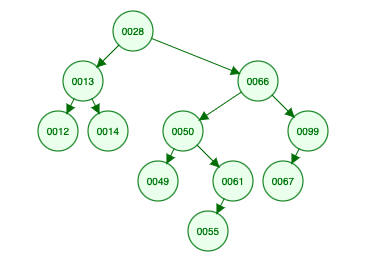
\includegraphics[width=1.2\linewidth]{Abbildungen/suchbaum}
			\caption{Binärer Suchbaum}
			\label{fig:suchbaum}
		\end{subfigure}%
		\begin{subfigure}{.5\textwidth}
			\centering
			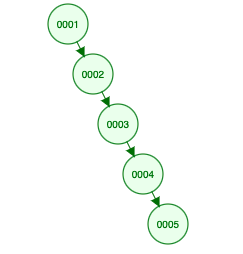
\includegraphics[width=0.7\linewidth]{Abbildungen/entartet}
			\caption{Entarteter Suchbaum}
			\label{fig:entartet}
		\end{subfigure}%
	\caption{Suchbäume}
	\end{figure}
	
	\subsection{Halden}
	\subsubsection*{Aufbau}
	Alle Nachfolger eines Knoten sind größter / kleiner (Min/Max Halde)
	\\'Ebenen' des Baumes werden von links nach rechts in Array eingebettet
		\begin{figure}[H]
			\centering
			\begin{subfigure}{.5\textwidth}
				\centering
				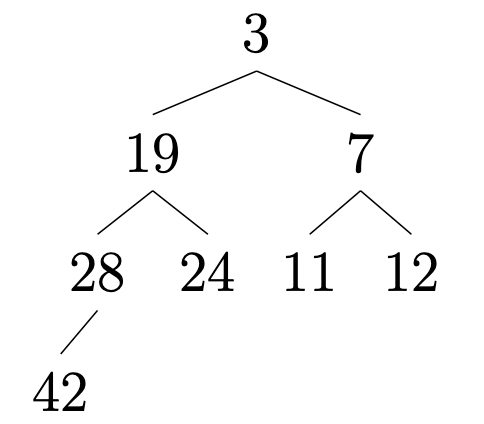
\includegraphics[width=.5\linewidth]{Abbildungen/halde}
				\caption{Min-Halde}
				\label{fig:halde}
			\end{subfigure}%
			\begin{subfigure}{.5\textwidth}
				\centering
				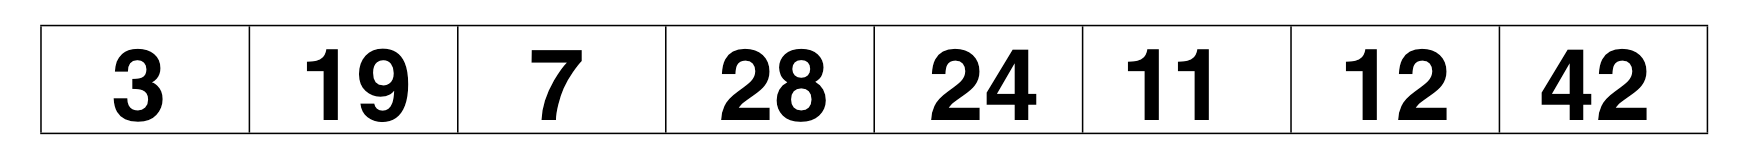
\includegraphics[width=0.7\linewidth]{Abbildungen/haldearr}
				\caption{Halde als Array}
				\label{fig:haldearr}
			\end{subfigure}%
			\caption{Halden}
		\end{figure}
	\subsubsection*{Einfügen}
	Neuen Wert hinten ins Array und dann Halden-Eigenschaft wiederherstellen:
	\\$\rightarrow$ Wert wird mit Elternknoten verglichen, bis Halden-Eigenschaft wieder gilt
	\subsubsection*{Löschen}
	Knoten löschen und letzten Wert im Array an Stelle bewegen
	\\dann Halden-Eigenschaft durch tauschen wiederherstellen
	
	\subsection{AVL-Bäume}
	\subsubsection*{Aufbau}
	Balancierte binäre Suchbäume
	\subsubsection*{Einfügen und Löschen}
	Analog zum Suchbaum
	\\mit darauffolgender Balancierphase
	\subsubsection{Balancieren}
	\textbf{Höhe}
	\\Anzahl Knoten unterhalb
	\\\textbf{Balancefaktor}
	\\$B = H_{links} - H_{rechts}$
	\\\textbf{Vorgehen bei der Klausur:} 
	\begin{enumerate}
		\item Höhe und Balancefaktor bei allen Knoten ermitteln
		\item Knoten mit $|B| \geq 2$ betrachten
		\item Vorzeichenwechsel? $\rightarrow$ 2 Rotationen
		\\sonst: eine Rotation
	\end{enumerate}
	\section{Graphen}
	\subsection{Begriffe}
	\begin{itemize}
		\item \textbf{Pfad}
		\\Weg zwischen zwei Knoten, Länge ist Anzahl von Kanten
		\item \textbf{Grad}
		\\Bei ungerichteten: Anzahl Verbindungen
		\\Bei gerichteten: Unterscheidung Eingangsgrad | Ausgangsgrad
		\item \textbf{Spannbaum}
		\\Zyklenfreier Teilgraph der alle Knoten enthält
		\item \textbf{Wurzel}
		\\Knoten mit Eingangsgrad 0
	\end{itemize}
	\subsection{Darstellungen}
	\subsubsection{TODO BILDER} %TODO Bilder
	\subsection{Spannbaum-Algorithmen}
	\subsubsection{Prim}
	\subsubsection{Kruskal}
	\subsection{TODO Tiefensuche Breitensuche, Algorithmen}
	\subsection{Traversierung}
	\subsubsection{Tiefensuche}
	Graph wird zu erst in die Tiefe durchsucht
	\\Würde ein bereits besuchter Knoten als nächstes kommen gehe einen Schritt zurück
	\begin{figure}[H]
		\centering
		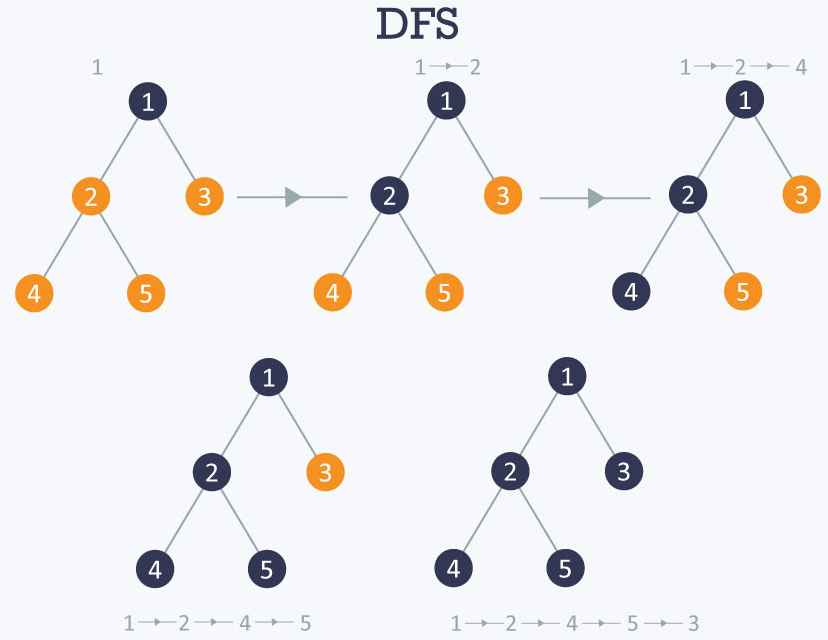
\includegraphics[width=0.7\linewidth]{Abbildungen/tiefensuche}
		\caption{Tiefensuche am Beispiel}
		\label{fig:tiefensuche}
	\end{figure}
	\textbf{Als Algorithmus:}
	\\Implementierung mit Stack
	\begin{itemize}
	\item Besuche Knoten
	\item Füge alle Kinder zu Stack hinzu
	\item Während Stack nicht empty:
	\item betrachte erstes Element von Stack, wenn noch nicht markiert: Punkt 1
	\end{itemize}

	\subsubsection{Breitensuche}
	Graph wird 'ebenenweise' durchsucht
	\\$\rightarrow$ Besuche erst alle Children, dann fange mit ihren Children an
\begin{figure}[H]
	\centering
	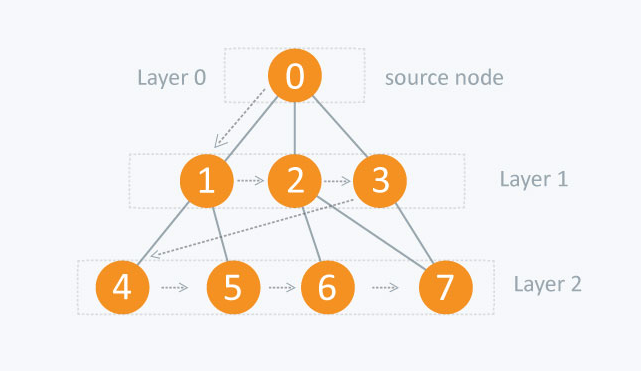
\includegraphics[width=0.5\linewidth]{Abbildungen/breitensuche}
	\caption{Breitensuche am Beispiel}
	\label{fig:breitensuche}
\end{figure}
	\textbf{Als Algorithmus:}
	\\Implementierung mit Queue
	\begin{itemize}
		\item Besuche Knoten
		\item Füge alle Children, die noch nicht besucht wurden,  in Queue hinzu
		\item Besuche nächsten Knoten in Queue
	\end{itemize}
	\subsection{Kürzeste Wege}
	\section{Rekursion}
	\section{Dyn. Prog.}
	\section{Sortieren}
	\section{HashMaps}
	\section{ADTs}
	\section{Listen}
	\section{Backtracking}
	\section{Suche}
	\section{WP-Kalk, Induktion}
	\section{Schreibtischlauf}
	\section{UML/OOP}
	\section{Vererbung}
\end{document}